% =============================================================
% Single-Image 3D Generation — A Comparative Evaluation
% Aram Abrahamyan · DS 235 · AUA · Spring 2026
%
% Rewritten in response to round-1 feedback:
%   1. Less text on every slide  -> bullets <=7 words, detail in \note{}.
%   2. 3D / NeRF terminology defined before use.
%   3. Every metric (NC, W, Sil-IoU, F-Score, ...) is defined before it appears in a result.
%   4. Each finding sits next to the number that supports it.
%   5. New property-based result slide (thickness / surface / material).
% =============================================================
\documentclass[aspectratio=169, 11pt]{beamer}

\usetheme{Madrid}
\usecolortheme{default}
\setbeamertemplate{navigation symbols}{}
\setbeamertemplate{footline}[frame number]

% ---- packages -----------------------------------------------
\usepackage{booktabs}
\usepackage{colortbl}
\usepackage{array}
\usepackage{tikz}
\usepackage{pgfplots}
\pgfplotsset{compat=1.18}
\usetikzlibrary{positioning, arrows.meta, shapes.geometric, fit, calc}
\usepackage{xcolor}
\usepackage{multirow}
\usepackage{graphicx}
\graphicspath{{figures/}{figures/qual_renders/}}

% ---- colour palette -----------------------------------------
\definecolor{tripocolor}{RGB}{31, 119, 180}
\definecolor{instantcolor}{RGB}{210, 95, 0}
\definecolor{sf3dcolor}{RGB}{34, 139, 34}
\definecolor{navydark}{RGB}{10, 28, 72}
\definecolor{warnfill}{RGB}{255, 248, 220}
\definecolor{warnborder}{RGB}{170, 115, 0}
\definecolor{goodfill}{RGB}{218, 245, 218}
\definecolor{goodborder}{RGB}{50, 135, 50}
\definecolor{infofill}{RGB}{220, 232, 255}
\definecolor{infoborder}{RGB}{55, 100, 185}
\definecolor{rowshade}{RGB}{244, 246, 252}
\definecolor{metup}{RGB}{0, 125, 52}
\definecolor{metdn}{RGB}{170, 28, 28}

\setbeamercolor{block title}{bg=navydark, fg=white}
\setbeamercolor{block body}{bg=navydark!7, fg=black}

% ---- arrow shorthand ----------------------------------------
\newcommand{\arrup}{\textcolor{metup}{$\uparrow$}}
\newcommand{\arrdn}{\textcolor{metdn}{$\downarrow$}}

% ---- coloured callouts --------------------------------------
\newcommand{\warncallout}[2][0.95\linewidth]{%
  \begin{tikzpicture}\node[fill=warnfill, draw=warnborder, line width=0.5pt,
        rounded corners=3pt, inner xsep=7pt, inner ysep=5pt,
        text width=#1, align=left, font=\scriptsize]
    {\textcolor{warnborder}{\textbf{$\blacktriangleright$}}\enspace #2};
  \end{tikzpicture}}
\newcommand{\goodcallout}[2][0.95\linewidth]{%
  \begin{tikzpicture}\node[fill=goodfill, draw=goodborder, line width=0.5pt,
        rounded corners=3pt, inner xsep=7pt, inner ysep=5pt,
        text width=#1, align=left, font=\scriptsize]
    {\textcolor{goodborder}{\textbf{$\checkmark$}}\enspace #2};
  \end{tikzpicture}}
\newcommand{\infocallout}[2][0.95\linewidth]{%
  \begin{tikzpicture}\node[fill=infofill, draw=infoborder, line width=0.5pt,
        rounded corners=3pt, inner xsep=7pt, inner ysep=5pt,
        text width=#1, align=left, font=\scriptsize]
    {\textcolor{infoborder}{\textbf{$\triangleright$}}\enspace #2};
  \end{tikzpicture}}

% ---- "metric -> finding" arrow row --------------------------
% \finding{metric line}{conclusion line}
\newcommand{\finding}[2]{%
  \begin{tikzpicture}
    \node[draw=navydark!50, fill=navydark!5, line width=0.4pt,
          rounded corners=3pt, inner sep=5pt,
          text width=0.93\linewidth, font=\scriptsize, align=left]
    {\textbf{#1}\\[1pt]\textcolor{navydark!80}{$\leadsto$}\enspace #2};
  \end{tikzpicture}\par}

\newcommand{\qimg}[1]{\includegraphics[width=1.6cm,height=1.6cm,keepaspectratio]{#1}}

% ---- title meta ---------------------------------------------
\title[Single-Image 3D Generation]{Single-Image 3D Generation\\
  \large A Comparative Evaluation of Three Feed-Forward Methods}
\author{Aram Abrahamyan}
\institute{DS 235 — Generative AI \quad·\quad American University of Armenia}
\date{Spring 2026}
\titlegraphic{
\includegraphics[height=1.4cm]{aua_logo.png}}

% Use the default beamer \note command (remove custom redefinition that caused errors).
% Hide notes during compilation to avoid note-related environment errors.
\setbeameroption{hide notes}
% =============================================================
\begin{document}

% -------------------------------------------------------------
\begin{frame}\titlepage\end{frame}

% =============================================================
% MOTIVATION
% =============================================================
\begin{frame}{Why single-image 3D matters}

  \begin{columns}[T]
    \column{0.55\textwidth}
      \textbf{Where 3D content is needed today}
      \vspace{0.5em}

      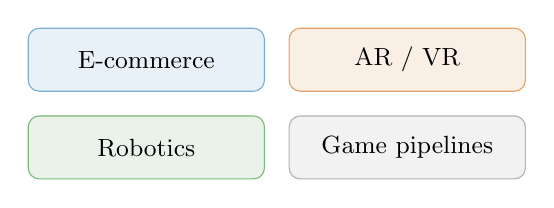
\begin{tikzpicture}[node distance=0.35cm]
        \node[draw=tripocolor!60, fill=tripocolor!10, rounded corners,
              minimum width=3.0cm, minimum height=0.8cm,
              font=\small, align=center] (ec)
              {E-commerce};
        \node[draw=instantcolor!60, fill=instantcolor!10, rounded corners,
              minimum width=3.0cm, minimum height=0.8cm,
              font=\small, align=center, right=0.3cm of ec] (ar)
              {AR / VR};
        \node[draw=sf3dcolor!60, fill=sf3dcolor!10, rounded corners,
              minimum width=3.0cm, minimum height=0.8cm,
              font=\small, align=center, below=0.3cm of ec] (rob)
              {Robotics};
        \node[draw=gray!60, fill=gray!10, rounded corners,
              minimum width=3.0cm, minimum height=0.8cm,
              font=\small, align=center, right=0.3cm of rob] (game)
              {Game pipelines};
      \end{tikzpicture}

    \column{0.42\textwidth}
      \begin{block}{Time to one asset}
        \scriptsize
        \begin{tabular}{lc}
          Manual artist & 4--8 \textbf{hours} \\
          Feed-forward model & $<$ \textbf{10 sec} \\
        \end{tabular}
      \end{block}

      \vspace{0.6em}
      \infocallout{\textbf{Question:} which feed-forward model should you actually use?}
  \end{columns}
  \note{%
    Single-image 3D is everywhere downstream:
    e-commerce previews, AR try-on, robot scene
    understanding, game asset pipelines. Manual modelling is hours;
    a feed-forward model is seconds. The interesting question is
    no longer ``can it work'' but ``which one should I pick'' --
    and that is what this evaluation answers.}
\end{frame}

% =============================================================
% TASK + AMBIGUITY
% =============================================================
\begin{frame}{The task: 1 image $\to$ 3D mesh}

  \begin{center}
  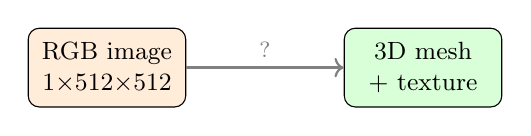
\begin{tikzpicture}[
      box/.style={draw, rounded corners, fill=blue!8,
                  minimum width=2.0cm, minimum height=1.0cm,
                  font=\small, align=center},
      arr/.style={->, thick, gray}]
    \node[box, fill=orange!15] (inp) {RGB image\\ $1{\times}512{\times}512$};
    \node[box, fill=green!15, right=2.0cm of inp] (out) {3D mesh\\ + texture};
    \draw[arr] (inp) -- (out) node[midway, above, font=\footnotesize] {?};
  \end{tikzpicture}
  \end{center}

  \vspace{0.4em}
  \begin{columns}[T]
    \column{0.32\textwidth}
      \centering
      \begin{block}{\small Depth ambiguity}
        \centering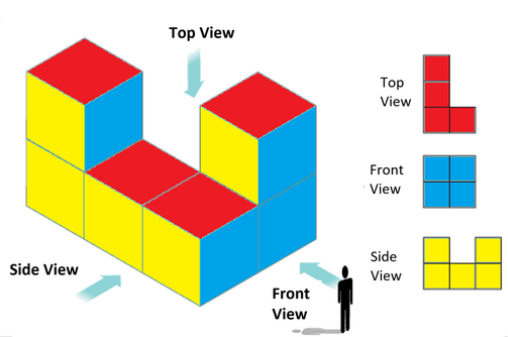
\includegraphics[height=2.0cm]{3d_ambiguity.png}\\[2pt]
        \scriptsize Many shapes project to the same image
      \end{block}
    \column{0.32\textwidth}
      \centering
      \begin{block}{\small The back is unseen}
        \centering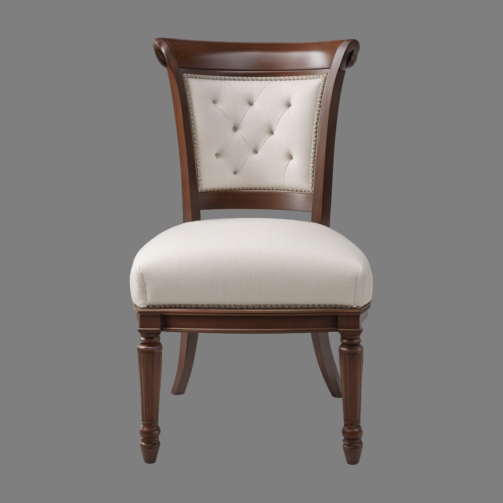
\includegraphics[height=2.0cm]{back_unobserved.png}\\[2pt]
        \scriptsize Half the surface is never observed
      \end{block}
    \column{0.32\textwidth}
      \centering
      \begin{block}{\small Texture vs.\ geometry}
        \centering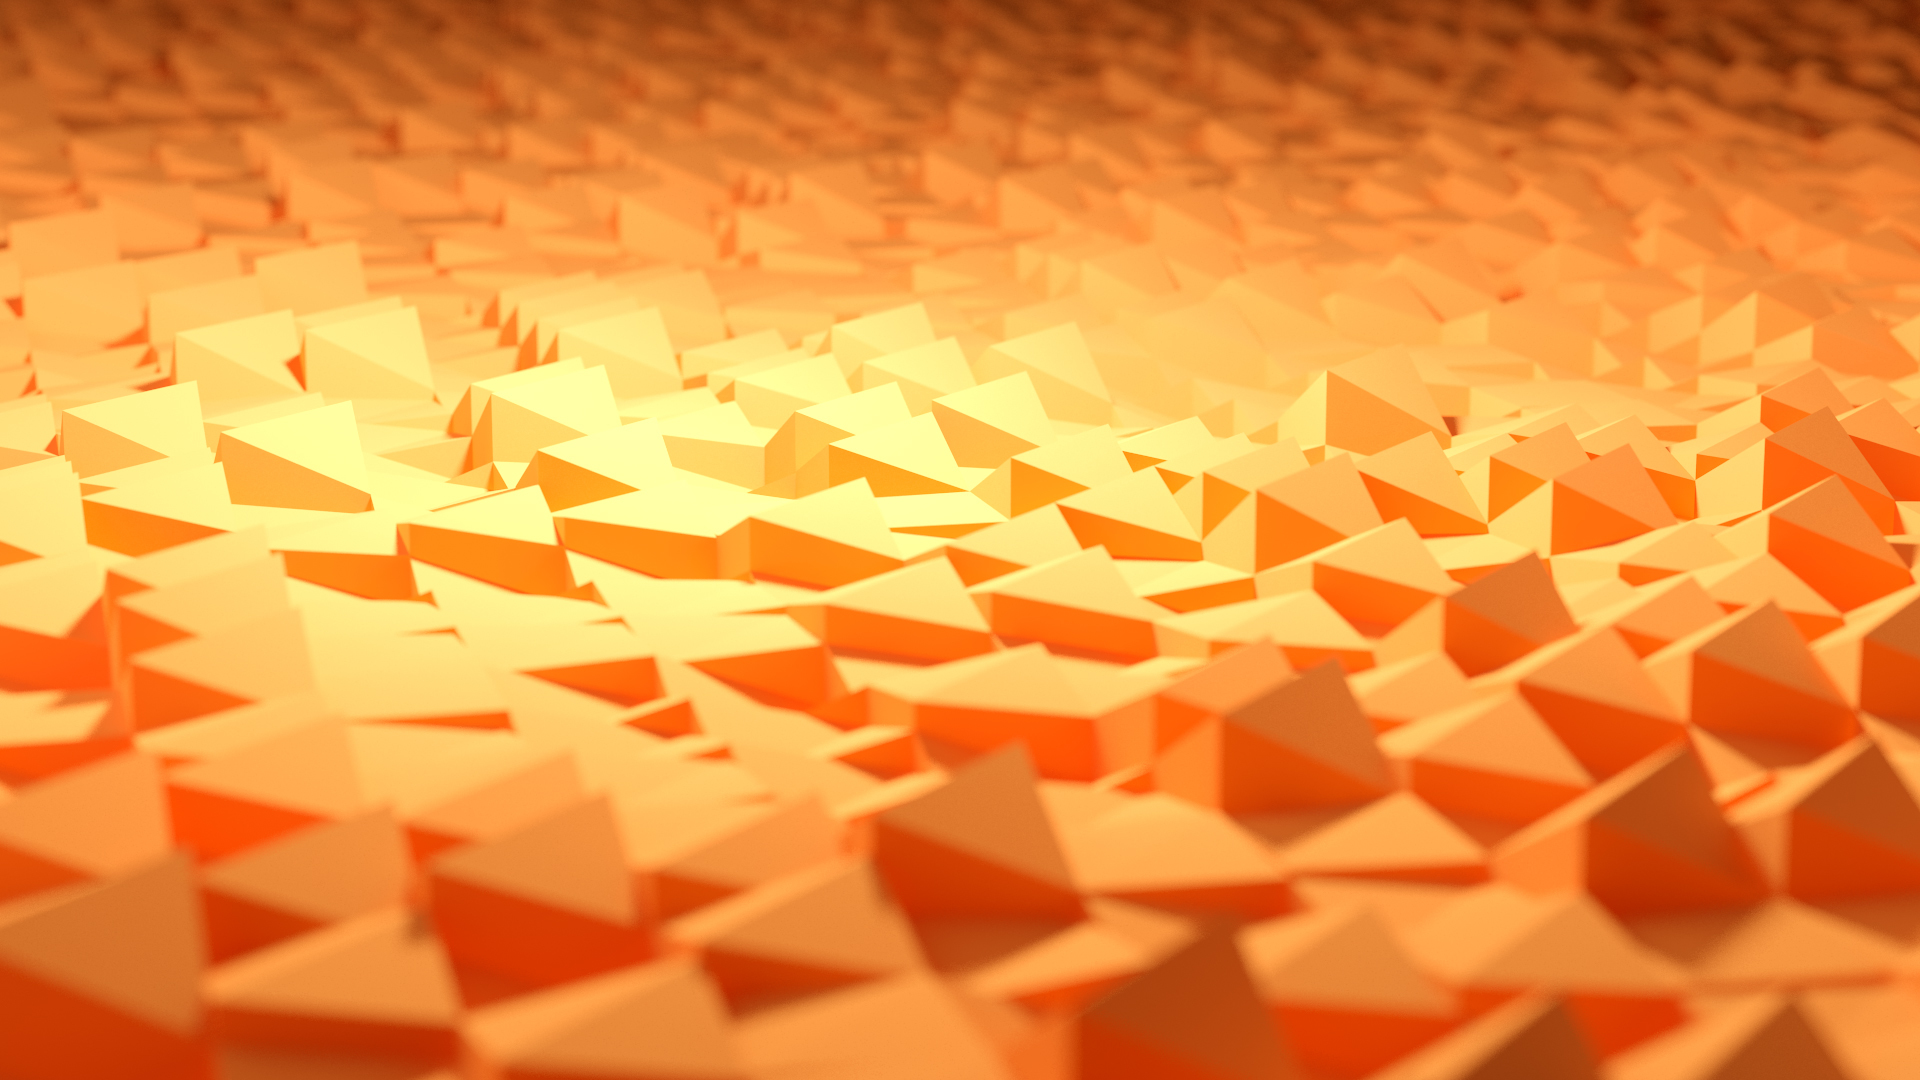
\includegraphics[height=2.0cm]{texture_vs_geometry.jpg}\\[2pt]
        \scriptsize Shadows can be mistaken for shape
      \end{block}
  \end{columns}
  \note{%
    The task is mathematically ill-posed: infinitely many 3-D
    shapes project to the same image. So every model has to make a
    \emph{prior} -- a guess about how the world tends to look. The
    three priors we compare are: (a) a NeRF density field
    (TripoSR), (b) hallucinate other views first (InstantMesh),
    (c) decompose into shape + material + lighting (SF3D).}
\end{frame}

% =============================================================
% 3D PRIMER  (NEW -- addresses feedback #2)
% =============================================================
\begin{frame}{3D primer: five terms used in this talk}

  \begin{columns}[T]
    \column{0.46\textwidth}
      \begin{block}{Mesh}
        \scriptsize Vertices $+$ triangle faces.\\
        Stores geometry; texture stored per-vertex or via UV map.
      \end{block}
      \begin{block}{NeRF MLP}
        \scriptsize A network mapping a 3-D point\\
        $(x,y,z) \to$ (density, colour).\\
        Mesh is extracted from the density field afterwards.
      \end{block}
      \begin{block}{Triplane}
        \scriptsize Three orthogonal 2-D feature grids ($XY, YZ, XZ$).\\
        Compactly encodes a 3-D scene; cheap lookup.
      \end{block}

    \column{0.50\textwidth}
      \begin{block}{Rendering}
        \scriptsize Project the 3-D representation\\
        from a chosen camera $\to$ 2-D image.
      \end{block}
      \begin{block}{Multi-view consistency}
        \scriptsize Render the same object from $N$ angles.\\
        If renders disagree (Janus heads, blank backs), \\
        the 3-D representation is incoherent.
      \end{block}

      \vspace{0.3em}
      \infocallout{\scriptsize That's everything you need. No 3D background assumed.}
  \end{columns}
  \note{%
    These five concepts are all the 3-D vocabulary any later slide
    will use. Mesh = the output. NeRF MLP and triplane = two ways
    to represent the geometry inside a model. Rendering = how we
    turn the representation back into pixels for evaluation.
    Multi-view consistency = the ``no Janus heads'' check we run
    afterwards.}
\end{frame}

% =============================================================
% LANDSCAPE
% =============================================================
\begin{frame}{Three methods, three priors}

  \begin{columns}[T]
    \column{0.50\textwidth}
      \centering
      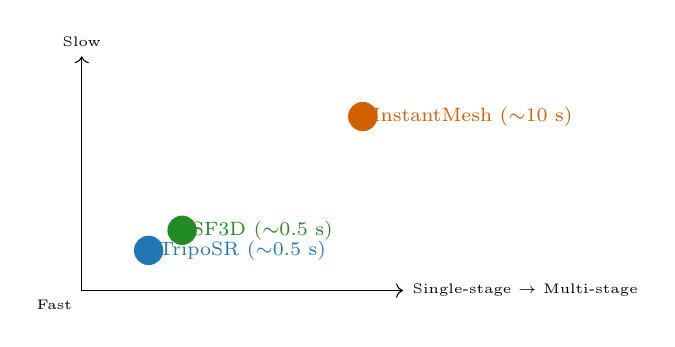
\begin{tikzpicture}[scale=0.85]
        \draw[->] (0,0) -- (4.8,0) node[right, font=\tiny] {Single-stage $\to$ Multi-stage};
        \draw[->] (0,0) -- (0,3.5) node[above, font=\tiny] {Slow};
        \node[font=\tiny, below left] at (0,0) {Fast};
        \filldraw[tripocolor]   (1.0, 0.6) circle (6pt)
              node[right, font=\scriptsize\color{tripocolor}] {TripoSR ($\sim$0.5 s)};
        \filldraw[sf3dcolor]    (1.5, 0.9) circle (6pt)
              node[right, font=\scriptsize\color{sf3dcolor}] {SF3D ($\sim$0.5 s)};
        \filldraw[instantcolor] (4.2, 2.6) circle (6pt)
              node[right, font=\scriptsize\color{instantcolor}] {InstantMesh ($\sim$10 s)};
      \end{tikzpicture}

    \column{0.46\textwidth}
      \scriptsize
      \renewcommand{\arraystretch}{1.3}
      \begin{tabular}{@{}lccc@{}}
        \toprule
                  & \textbf{TripoSR} & \textbf{InstantMesh} & \textbf{SF3D} \\
        \midrule
        Year      & 2024 & 2024 & 2025 \\
        Paradigm  & LRM & Diff $+$ LRM & LRM $+$ MatNet \\
        Output    & vertex colour & vertex colour & UV $+$ PBR \\
        Speed     & $\sim$0.5 s & $\sim$10 s & $\sim$0.5 s \\
        \bottomrule
      \end{tabular}
  \end{columns}

  \vspace{0.6em}
  \scriptsize
  \textbf{LRM} = large reconstruction model (a transformer that maps an image to a 3-D representation in one pass).\\
  \textbf{PBR} = physically-based rendering — the asset has separate albedo / roughness / metallic maps so it can be \emph{relit}.
  \note{%
    Feed-forward LRM is a transformer that ingests an image and
    produces the 3-D scene tokens directly. The three methods
    differ in (1) whether they hallucinate other views first,
    (2) whether they predict material maps. TripoSR is the
    minimal version; InstantMesh trades latency for quality;
    SF3D trades absolute geometry for production-ready output.}
\end{frame}

% =============================================================
% TRIPOSR
% =============================================================
\begin{frame}{TripoSR — single-stage triplane $\to$ NeRF}

  \begin{center}
  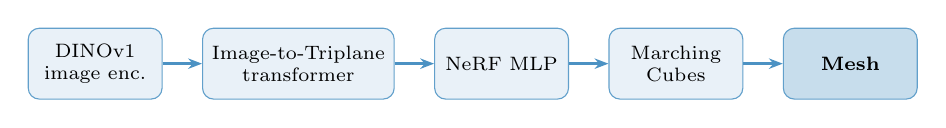
\begin{tikzpicture}[
      box/.style={draw=tripocolor!70, fill=tripocolor!10, rounded corners=4pt,
                  minimum width=1.7cm, minimum height=0.9cm,
                  font=\scriptsize, align=center},
      arr/.style={-{Stealth[length=5pt]}, line width=1.0pt, tripocolor!80}]
    \node[box] (enc)  {DINOv1\\image enc.};
    \node[box, right=0.5cm of enc]  (tr)   {Image-to-Triplane\\transformer};
    \node[box, right=0.5cm of tr]   (nerf) {NeRF MLP};
    \node[box, right=0.5cm of nerf] (mc)   {Marching\\Cubes};
    \node[box, right=0.5cm of mc, fill=tripocolor!25]   (mesh) {\textbf{Mesh}};
    \draw[arr] (enc)--(tr); \draw[arr] (tr)--(nerf);
    \draw[arr] (nerf)--(mc); \draw[arr] (mc)--(mesh);
  \end{tikzpicture}
  \end{center}

  \begin{columns}[T]
    \column{0.55\textwidth}
      \scriptsize
      \begin{itemize}
        \item DINOv1 ViT $\to$ image tokens
        \item Cross-attention $\to$ $64{\times}64$ triplane
        \item NeRF MLP reads density $+$ colour
        \item Marching cubes $\to$ vertex-coloured mesh
      \end{itemize}

    \column{0.41\textwidth}
      \warncallout{$64^2$ triplane is coarse $\to$ aliases on thin parts. No material model.}
  \end{columns}
  \note{%
    TripoSR is the simplest of the three. Image goes in, a single
    transformer turns it into a triplane, a small MLP reads
    density and RGB from the triplane (this is the NeRF), and
    marching cubes extracts a mesh. No multi-view, no material.
    This means it is fast and small, and we will see this
    purity helps it on simple objects but hurts it on thin or
    metallic ones.}
\end{frame}

% =============================================================
% INSTANTMESH
% =============================================================
\begin{frame}{InstantMesh — hallucinate views, then reconstruct}

  \begin{center}
    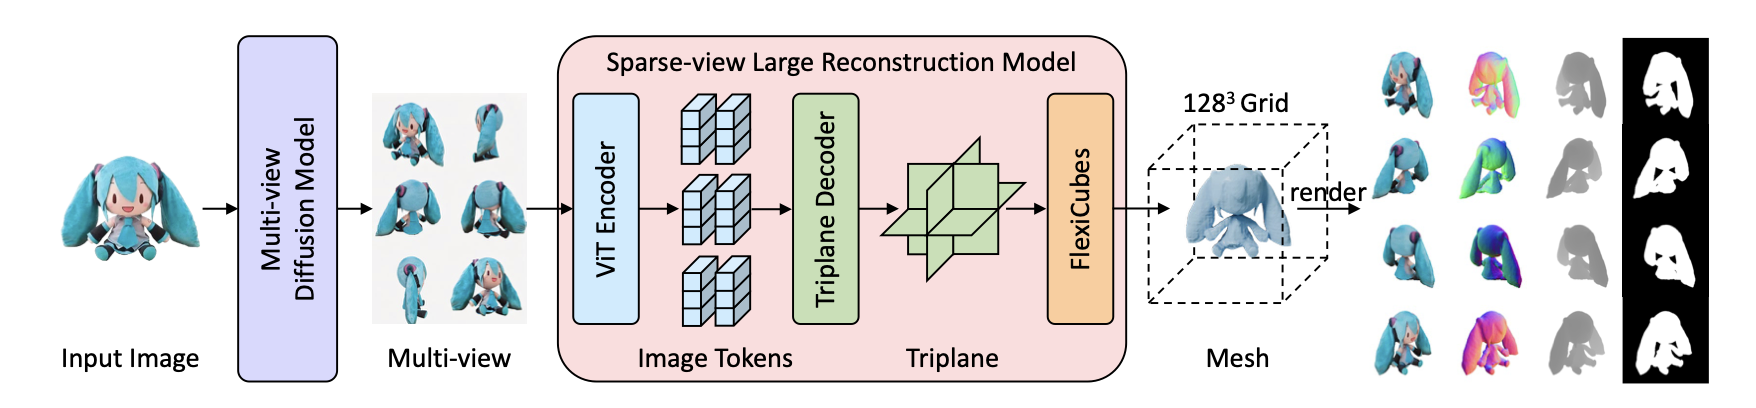
\includegraphics[width=0.78\linewidth]{instantmesh_architecture.png}
  \end{center}

  \begin{columns}[T]
    \column{0.55\textwidth}
      \scriptsize
      \begin{itemize}
        \item Stage 1: Zero123$++$ diffusion $\to$ \textbf{6 novel views}
        \item Stage 2: sparse-view LRM $\to$ mesh
        \item FlexiCubes iso-surface $+$ depth $/$ normal supervision
        \item End-to-end $\sim$10 s; only watertight method here
      \end{itemize}

    \column{0.41\textwidth}
      \warncallout{Diffusion can disagree with itself $\to$ noise propagates into geometry. $\sim$20$\times$ slower.}
  \end{columns}
  \note{%
    InstantMesh is two stages. First, a fine-tuned Zero123++
    diffusion model takes the input image and synthesises six
    novel views from canonical angles. Second, a sparse-view LRM
    consumes all six views (plus the input) and outputs a mesh.
    The iso-surface step is FlexiCubes -- a differentiable
    marching-cubes variant that lets the model apply geometric
    losses on the mesh directly. Watertight outputs come from
    here.}
\end{frame}

% =============================================================
% SF3D
% =============================================================
\begin{frame}{SF3D — geometry $+$ material $+$ lighting}

  \begin{center}
    
\includegraphics[width=0.65\linewidth]{sf3d.png}
  \end{center}

  \begin{columns}[T]
    \column{0.55\textwidth}
      \scriptsize
      \begin{itemize}
        \item Higher-resolution triplane (vs.\ TripoSR)
        \item \textbf{MaterialNet:} albedo / roughness / metallic
        \item \textbf{LightNet:} estimates illumination
        \item Vertex offsets smooth the iso-surface
        \item UV unwrap $\to$ PBR-ready GLB
      \end{itemize}

    \column{0.41\textwidth}
      \goodcallout{Only method whose output is directly drop-in into a renderer / game engine. CVPR'25.}
  \end{columns}
  \note{%
    SF3D adds two heads on top of a TripoSR-like backbone:
    MaterialNet predicts surface material parameters per point,
    and LightNet predicts the ambient illumination. The asset
    can therefore be re-lit: you can drop it into a different
    scene and it shades correctly. The downside is that the
    model spends capacity on material/lighting that the other
    two spend on raw geometry.}
\end{frame}

% =============================================================
% EVAL SETUP
% =============================================================
\begin{frame}{How we evaluate (one input, three pipelines, same metrics)}

  \begin{center}
  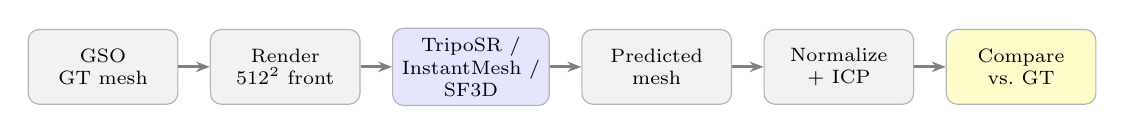
\begin{tikzpicture}[
      box/.style={draw=gray!60, fill=gray!10, rounded corners=4pt,
                  minimum width=1.9cm, minimum height=0.95cm,
                  font=\scriptsize, align=center},
      arr/.style={-{Stealth[length=5pt]}, line width=1.0pt, gray}]
    \node[box] (gso)  {GSO\\GT mesh};
    \node[box, right=0.4cm of gso]  (rend) {Render\\$512^2$ front};
    \node[box, right=0.4cm of rend, fill=blue!10] (mod)  {TripoSR /\\InstantMesh /\\SF3D};
    \node[box, right=0.4cm of mod]  (pred) {Predicted\\mesh};
    \node[box, right=0.4cm of pred] (aln)  {Normalize\\$+$ ICP};
    \node[box, right=0.4cm of aln, fill=yellow!20]  (cmp)  {Compare\\vs.\ GT};
    \draw[arr](gso)--(rend); \draw[arr](rend)--(mod);
    \draw[arr](mod)--(pred); \draw[arr](pred)--(aln);
    \draw[arr](aln)--(cmp);
  \end{tikzpicture}
  \end{center}

  \vspace{0.6em}
  \begin{columns}[T]
    \column{0.48\textwidth}
      \begin{block}{Dataset}
        \scriptsize
        \textbf{100 objects} from Google Scanned Objects.\\
        Categories: household, apparel, electronics, toys, packaging.
      \end{block}
    \column{0.48\textwidth}
      \begin{block}{Pipeline}
        \scriptsize
        Render canonical front view $\to$ feed all three models.\\
        Both meshes normalized to unit bbox $\to$ 24-rotation search $\to$ ICP.
      \end{block}
  \end{columns}
  \note{%
    We render one canonical front view of each GSO object at
    $512{\times}512$ on a white background. The exact same image is
    fed to all three models. We then evaluate each predicted mesh
    against the GSO ground-truth mesh after centring and rescaling
    both to a unit bounding-box diagonal. This makes Chamfer and
    F-score scale-invariant.}
\end{frame}

% =============================================================
% METRICS PRIMER 1  (NEW -- addresses feedback #3)
% =============================================================
\begin{frame}{Metrics — image \& alignment}
  \scriptsize
  \renewcommand{\arraystretch}{1.45}
  \begin{tabular}{@{}p{2.8cm}cp{8.6cm}@{}}
    \toprule
    \textbf{Metric} & \textbf{Dir.} & \textbf{Definition} \\
    \midrule
    PSNR & \arrup &
      $10\,\log_{10}(1/\mathrm{MSE})$ between front render and input — pixel match. \\
    SSIM & \arrup &
      Structural similarity in local windows; robust to small misalignments. \\
    LPIPS & \arrdn &
      Distance in AlexNet feature space — best correlates with human texture judgement. \\
    CLIP-sim & \arrup &
      Cosine of CLIP embeddings (input vs.\ render) — \emph{semantic} identity match. \\
    \textbf{Sil-IoU} & \arrup &
      Silhouette IoU: $|\hat S \cap S_{\text{in}}| / |\hat S \cup S_{\text{in}}|$.
      Catches \emph{scale / pose} mismatches that pixel metrics miss. \\
    \textbf{Multi-view CLIP} & \arrup &
      Mean CLIP similarity across $N{=}8$ rendered views. Low $\Rightarrow$ Janus heads, blank backs. \\
    \bottomrule
  \end{tabular}
  \note{%
    Six metrics, two questions. The first four (PSNR/SSIM/LPIPS/CLIP)
    ask: ``does the front render look like the input?'' --
    pixel-level, structural, perceptual, semantic respectively.
    Sil-IoU asks the orthogonal question: ``is the predicted mesh
    in the right place / scale at all?'' Multi-view CLIP renders the
    object from 8 angles and asks ``do the views agree with each
    other?'' -- our reference-free check for coherent 3-D output.}
\end{frame}

% =============================================================
% METRICS PRIMER 2
% =============================================================
\begin{frame}{Metrics — geometry vs.\ ground truth}
  \scriptsize
  \renewcommand{\arraystretch}{1.45}
  \begin{tabular}{@{}p{3.1cm}cp{8.3cm}@{}}
    \toprule
    \textbf{Metric} & \textbf{Dir.} & \textbf{Definition} (after both meshes are normalized to unit bbox) \\
    \midrule
    \textbf{Chamfer-L1} & \arrdn &
      $\overline{d}_{p\to r} + \overline{d}_{r\to p}$, i.e.\ mean nearest-neighbour distance both ways
      between sampled point clouds. Sensitive to outliers. \\
    \textbf{F-Score @ $\tau$} & \arrup &
      Sample point matched if it is within $\tau$ of the other surface; report F1 of precision/recall.
      We use $\tau \in \{1\%, 2\%, 5\%\}$ of the bbox diagonal. \\
    \textbf{NC} (normal consistency) & \arrup &
      $\tfrac12\big(\mathbb{E}|\cos\theta_{p\to r}| + \mathbb{E}|\cos\theta_{r\to p}|\big)$
      where $\theta$ is the angle between matched face normals.
      \emph{Surfaces face the same way}, not just sit close. \\
    \textbf{W \%} (watertight) & \arrup &
      Fraction of meshes that are closed manifolds. Required for volume / 3-D printing / fluid sim. \\
    \bottomrule
  \end{tabular}

  \vspace{0.6em}
  \infocallout{We always report both Chamfer \emph{and} F-Score: a few stray vertices wreck Chamfer; F-Score is robust to that.}
  \note{%
    These four define "geometry quality". Chamfer is mean
    distance, so a single bad vertex spikes it. F-Score thresholds
    that distance and counts -- robust. Normal consistency is
    crucial: two surfaces can be Chamfer-close but face the wrong
    way (think of a thin sheet versus its mirror -- close in
    distance, opposite in normals). Watertight is binary per mesh
    -- needed for any downstream that requires a sealed surface.}
\end{frame}

% =============================================================
% RESULTS — GEOMETRY
% =============================================================
\begin{frame}{Results — geometry vs.\ GT ($n{=}100$)}

  \begin{columns}[T]
    \column{0.58\textwidth}
      \centering\scriptsize
      \renewcommand{\arraystretch}{1.3}
      \begin{tabular}{@{}lccccc@{}}
        \toprule
        \textbf{Method} & \textbf{CD\,\arrdn} & \textbf{F@1\%\,\arrup} & \textbf{F@2\%\,\arrup} & \textbf{NC\,\arrup} & \textbf{W\%\,\arrup} \\
        \midrule
        \rowcolor{tripocolor!8}
        \textcolor{tripocolor}{\textbf{TripoSR}}
          & \textbf{0.129} & 0.134 & 0.257 & \textbf{0.642} & 0\,\% \\
        \rowcolor{instantcolor!8}
        \textcolor{instantcolor}{\textbf{InstantMesh}}
          & 0.132 & \textbf{0.152} & \textbf{0.275} & 0.627 & \textbf{38\,\%} \\
        \rowcolor{sf3dcolor!8}
        \textcolor{sf3dcolor}{\textbf{SF3D}}
          & 0.185 & 0.084 & 0.166 & 0.526 & 0\,\% \\
        \bottomrule
      \end{tabular}
      \vspace{0.3em}
      \tiny CD = Chamfer-L1 (unit-bbox); NC = normal consistency; W\% = watertight fraction.

      \vspace{0.7em}
      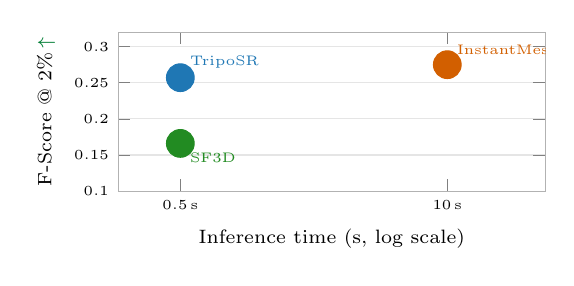
\begin{tikzpicture}
      \begin{axis}[
        width=7.0cm, height=3.6cm,
        xlabel={\scriptsize Inference time (s, log scale)},
        ylabel={\scriptsize F-Score @ 2\%\,\arrup},
        xmode=log, xtick={0.5, 10},
        xticklabels={$0.5$\,s, $10$\,s},
        ymin=0.10, ymax=0.32, xmin=0.25, xmax=30,
        ymajorgrids=true, grid style={gray!20},
        tick label style={font=\tiny},
        label style={font=\scriptsize},
        axis line style={gray!60},
      ]
        \addplot[only marks, mark=*, mark size=5pt, color=tripocolor]
          coordinates {(0.5, 0.257)};
        \node[font=\tiny, color=tripocolor, anchor=south west]
          at (axis cs:0.5, 0.257) {TripoSR};
        \addplot[only marks, mark=*, mark size=5pt, color=instantcolor]
          coordinates {(10, 0.275)};
        \node[font=\tiny, color=instantcolor, anchor=south west]
          at (axis cs:10, 0.275) {InstantMesh};
        \addplot[only marks, mark=*, mark size=5pt, color=sf3dcolor]
          coordinates {(0.5, 0.166)};
        \node[font=\tiny, color=sf3dcolor, anchor=north west]
          at (axis cs:0.5, 0.166) {SF3D};
      \end{axis}
      \end{tikzpicture}

    \column{0.40\textwidth}
      \finding{F@2\,\%: \textbf{InstantMesh 0.275}}{Multi-view diffusion sees 6 hallucinated views $\Rightarrow$ recovers occluded surfaces.}\vspace{0.2em}
      \finding{Chamfer / NC: \textbf{TripoSR wins}}{Single coherent NeRF density $\Rightarrow$ no view-aggregation artefacts.}\vspace{0.2em}
      \finding{W\,\%: \textbf{InstantMesh 38\,\%}}{FlexiCubes outputs closed manifolds; the other two extract via marching cubes and leak holes.}\vspace{0.2em}
      \finding{All scores low, F@1\,\%: \textbf{0.08--0.15}}{Single-image 3D is still hard at strict thresholds.}
  \end{columns}
  % \note{%
  %   The headline geometry numbers. TripoSR has the best mean
  %   surface distance and the best normal alignment; InstantMesh
  %   has the best F-scores at every threshold, by hallucinating
  %   extra views; SF3D loses on raw geometry because it splits its
  %   capacity with material and lighting. Every method's F-score at
  %   1\% is below 0.15 -- single-image 3-D from one view is still
  %   far from solved at strict tolerance.}
\end{frame}
% =============================================================

% =============================================================
% RESULTS — APPEARANCE / ALIGNMENT
% =============================================================
\begin{frame}{Results — appearance \& alignment ($n{=}100$)}

  \begin{columns}[T]
    \column{0.58\textwidth}
      \centering\scriptsize
      \renewcommand{\arraystretch}{1.3}
      \begin{tabular}{@{}lcccccc@{}}
        \toprule
        \textbf{Method} & \textbf{PSNR\,\arrup} & \textbf{SSIM\,\arrup} & \textbf{LPIPS\,\arrdn} & \textbf{CLIP\,\arrup} & \textbf{Sil-IoU\,\arrup} & \textbf{MV\,\arrup} \\
        \midrule
        \rowcolor{tripocolor!8}
        \textcolor{tripocolor}{\textbf{TripoSR}}
          & 11.19 & \textbf{0.756} & \textbf{0.455} & 0.706 & 0.104 & 0.903 \\
        \rowcolor{instantcolor!8}
        \textcolor{instantcolor}{\textbf{InstantMesh}}
          & 11.15 & 0.727 & 0.507 & 0.680 & 0.119 & 0.897 \\
        \rowcolor{sf3dcolor!8}
        \textcolor{sf3dcolor}{\textbf{SF3D}}
          & \textbf{11.31} & 0.731 & 0.491 & \textbf{0.708} & \textbf{0.271} & \textbf{0.917} \\
        \bottomrule
      \end{tabular}

      \vspace{0.7em}
      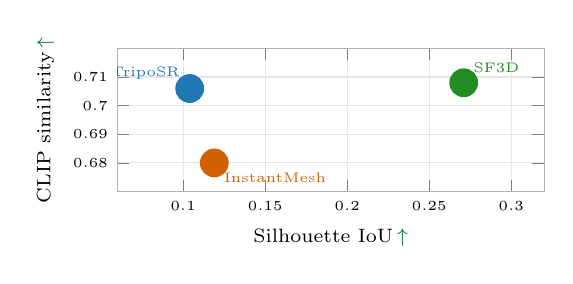
\begin{tikzpicture}
      \begin{axis}[
        width=7.0cm, height=3.4cm,
        xlabel={\scriptsize Silhouette IoU\,\arrup},
        ylabel={\scriptsize CLIP similarity\,\arrup},
        ymin=0.670, ymax=0.720,
        xmin=0.06,  xmax=0.32,
        ymajorgrids=true, xmajorgrids=true,
        grid style={gray!20},
        tick label style={font=\tiny},
        label style={font=\scriptsize},
        axis line style={gray!60},
        ytick={0.68, 0.69, 0.70, 0.71},
        xtick={0.10, 0.15, 0.20, 0.25, 0.30},
      ]
        \addplot[only marks, mark=*, mark size=5pt, color=tripocolor]
          coordinates {(0.104, 0.706)};
        \node[font=\tiny, color=tripocolor, anchor=south east]
          at (axis cs:0.104, 0.706) {TripoSR};
        \addplot[only marks, mark=*, mark size=5pt, color=instantcolor]
          coordinates {(0.119, 0.680)};
        \node[font=\tiny, color=instantcolor, anchor=north west]
          at (axis cs:0.119, 0.680) {InstantMesh};
        \addplot[only marks, mark=*, mark size=5pt, color=sf3dcolor]
          coordinates {(0.271, 0.708)};
        \node[font=\tiny, color=sf3dcolor, anchor=south west]
          at (axis cs:0.271, 0.708) {SF3D};
      \end{axis}
      \end{tikzpicture}

    \column{0.40\textwidth}
      \finding{Sil-IoU: \textbf{SF3D 0.27} (2.5$\times$ others)}{UV-PBR pipeline preserves the input scale; others routinely produce mesh that is wrong size or pose.}\vspace{0.2em}
      \finding{LPIPS / SSIM: \textbf{TripoSR}}{Coherent NeRF $\Rightarrow$ smoother textures and structures pixel-by-pixel.}\vspace{0.2em}
      \finding{MV CLIP: \textbf{SF3D 0.917}}{Most coherent from all sides.}\vspace{0.2em}
      \finding{CLIP-sim front: \textbf{tied SF3D / TripoSR}}{Object identity preserved across all three.}
  \end{columns}
  % \note{%
  %   Appearance / alignment. SF3D's silhouette-IoU win is the most
  %   important number on this slide -- 2.5x the other two -- and
  %   explains the otherwise puzzling fact that SF3D loses geometry
  %   metrics yet feels right when you look at the output: the mesh
  %   sits in the right pose. TripoSR keeps the LPIPS / SSIM
  %   advantage from a coherent representation. PSNR is uniformly
  %   low across the board because all three models warp the image
  %   plane slightly, and PSNR is unforgiving to that.}
\end{frame}

% =============================================================
% PROPERTY-BASED  (NEW -- addresses feedback #6)
% =============================================================
\begin{frame}{Property-based slice — 30 hand-labelled objects}

  \begin{columns}[T]
    \column{0.62\textwidth}
      \scriptsize
      \textbf{F-Score @ 2\,\% (\arrup), by surface type}
      \vspace{0.2em}

      \renewcommand{\arraystretch}{1.3}
      \begin{tabular}{@{}lcccc@{}}
        \toprule
        \textbf{Surface} & $n$ & \textbf{TripoSR} & \textbf{InstantMesh} & \textbf{SF3D} \\
        \midrule
        smooth    & 11 & \textbf{0.329} & 0.273 & 0.129 \\
        textured  &  8 & 0.279 & \textbf{0.411} & 0.146 \\
        detailed  & 11 & \textbf{0.244} & 0.227 & 0.168 \\
        \bottomrule
      \end{tabular}

      \vspace{0.6em}
      \textbf{LPIPS (\arrdn), by material}
      \begin{tabular}{@{}lcccc@{}}
        \toprule
        \textbf{Material} & $n$ & \textbf{TripoSR} & \textbf{InstantMesh} & \textbf{SF3D} \\
        \midrule
        matte   & 16 & \textbf{0.378} & 0.439 & 0.413 \\
        glossy  & 11 & \textbf{0.428} & 0.481 & 0.474 \\
        mixed   &  3 & \textbf{0.558} & 0.616 & 0.585 \\
        \bottomrule
      \end{tabular}

    \column{0.36\textwidth}
      \finding{\textbf{Textured surface} $\to$ InstantMesh}{0.411 vs.\ 0.279 / 0.146 — printed-graphics packaging hits the multi-view diffusion sweet spot.}\vspace{0.2em}
      \finding{\textbf{Smooth / detailed} $\to$ TripoSR}{Coherent NeRF generalises to ``generic'' shapes.}\vspace{0.2em}
      \finding{\textbf{Mixed (metallic, $n{=}3$)} $\to$ all fail}{LPIPS $\sim 0.6$ across the board; specular cues confuse every method.}
  \end{columns}

  \vspace{0.3em}
  \tiny Subset: 30/100 objects hand-labelled in \texttt{data/property\_labels.csv}.
  Full breakdown across thickness $/$ surface $/$ material in \texttt{runs/eval/by\_property.md}.
\end{frame}

% =============================================================
% QUALITATIVE
% =============================================================
\begin{frame}{Qualitative — three objects, three stories}

  \begin{center}
  \footnotesize
  \setlength{\tabcolsep}{4pt}
  \renewcommand{\arraystretch}{1.0}
  \begin{tabular}{@{}c|cccc@{}}
    \toprule
    \textbf{Object} & \textbf{Input} &
    \textcolor{tripocolor}{\textbf{TripoSR}} &
    \textcolor{instantcolor}{\textbf{InstantMesh}} &
    \textcolor{sf3dcolor}{\textbf{SF3D}} \\
    \midrule
    \rowcolor{rowshade}
    \scriptsize Elephant (organic)
      & \qimg{qual_renders/elephant/input.png}
      & \qimg{elephant_triposr.png}
      & \qimg{elephant_instantmesh.png}
      & \qimg{elephant_sf3d.png} \\[0.2em]
    \scriptsize Dragon (complex)
      & \qimg{qual_renders/dragon/input.png}
      & \qimg{dragon_triposr.png}
      & \qimg{dragon_instantmesh.png}
      & \qimg{dragon_sf3d.png} \\[0.2em]
    \rowcolor{rowshade}
    \scriptsize Toaster (metallic)
      & \qimg{qual_renders/toaster/input.png}
      & \qimg{toaster_triposr.png}
      & \qimg{toaster_instantmesh.png}
      & \qimg{toaster_sf3d.png} \\
    \bottomrule
  \end{tabular}
  \end{center}
  \note{%
    Quick visual confirmation. Elephant: organic, all three handle
    it. Dragon: complex shape with thin parts, InstantMesh's
    multi-view stage helps but introduces a slight blur; SF3D
    smooths thin parts away. Toaster: metallic and reflective --
    none of the three reconstruct the chrome correctly; SF3D's
    material model misfires; TripoSR baked the reflections into
    geometry. The qualitative pattern matches the
    property-based numbers on the previous slide.}
\end{frame}

% =============================================================
% FAILURE MODES
% =============================================================
\begin{frame}{Predictable failure modes}

  \begin{columns}[T]
    \column{0.32\textwidth}
      \begin{block}{\color{tripocolor}TripoSR}
        \centering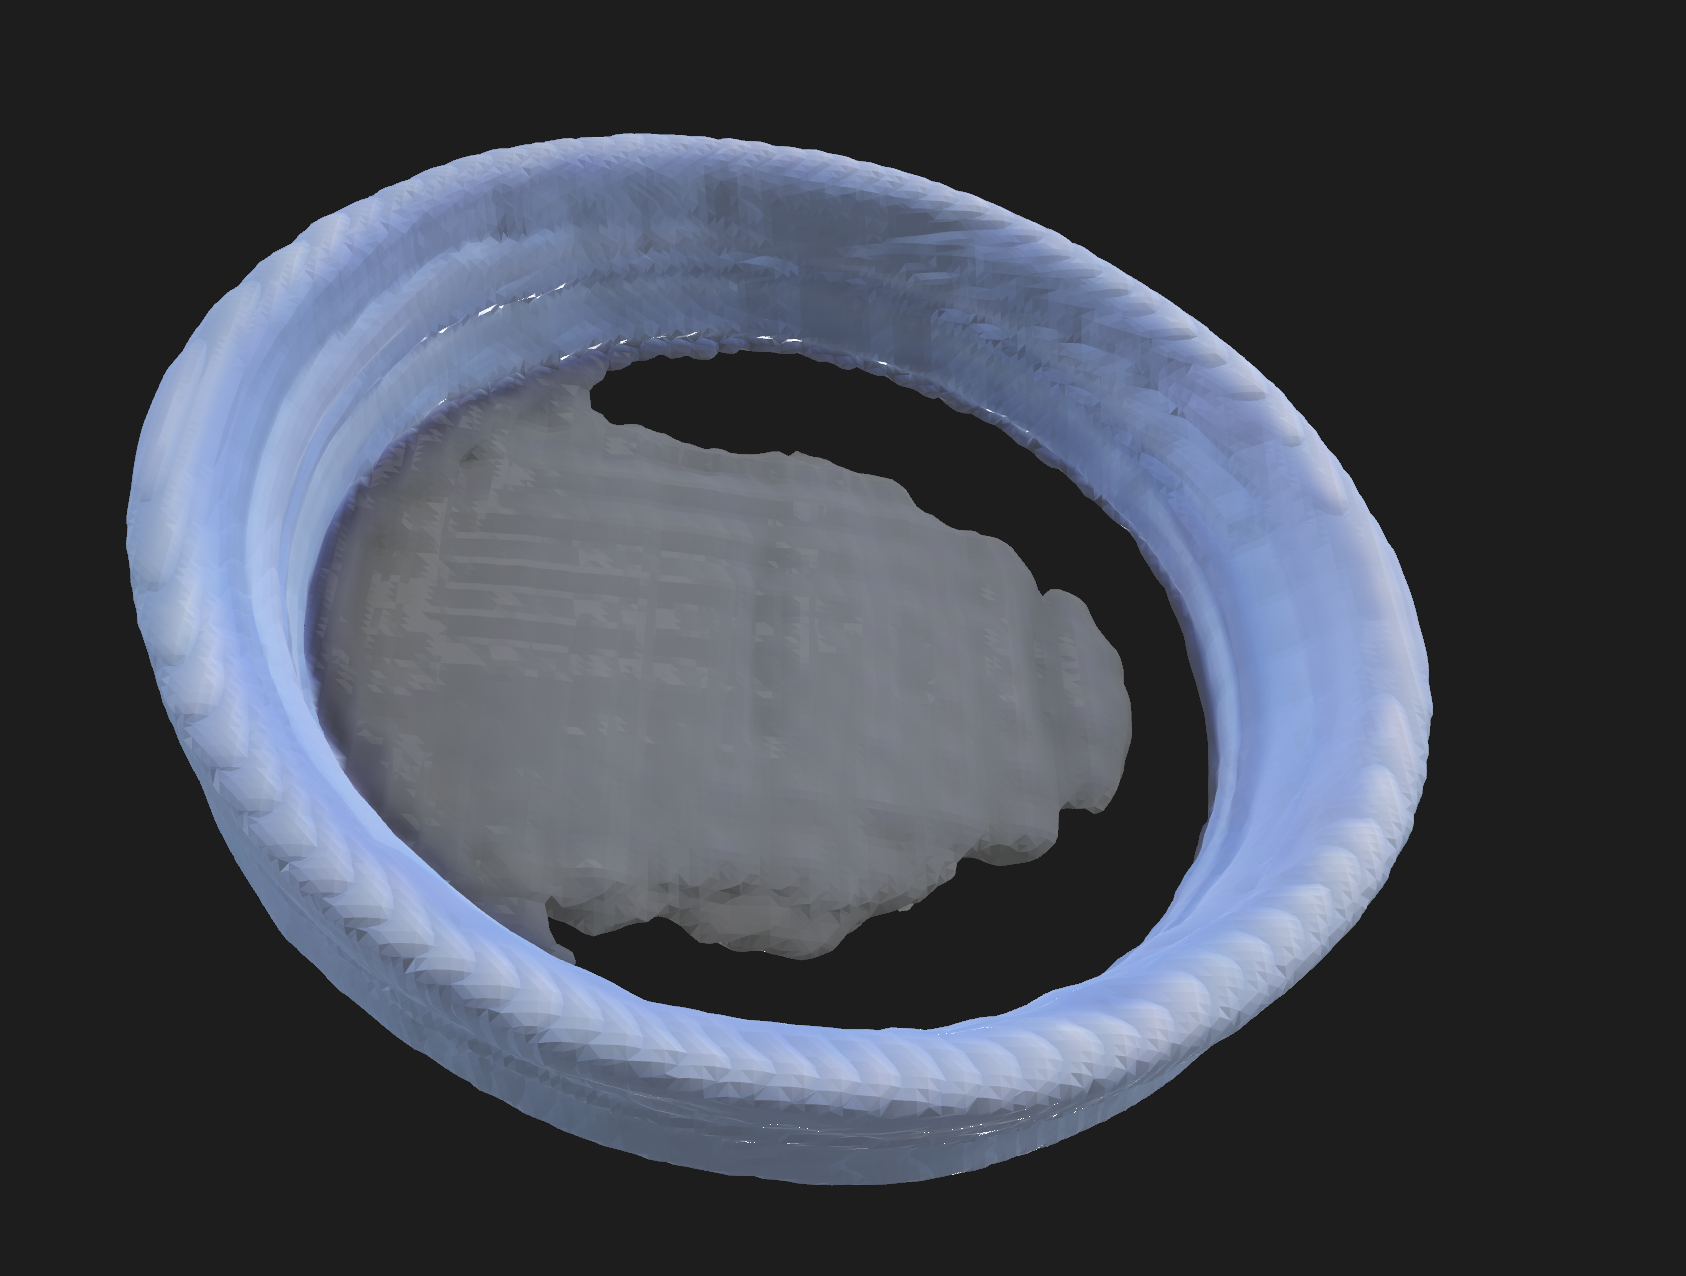
\includegraphics[height=2.2cm]{tripoSR_failure_case.png}\\[2pt]
        \scriptsize \textbf{Thin structures}\\$64^2$ triplane smooths fork tines / wire away.
      \end{block}
    \column{0.32\textwidth}
      \begin{block}{\color{instantcolor}InstantMesh}
        \centering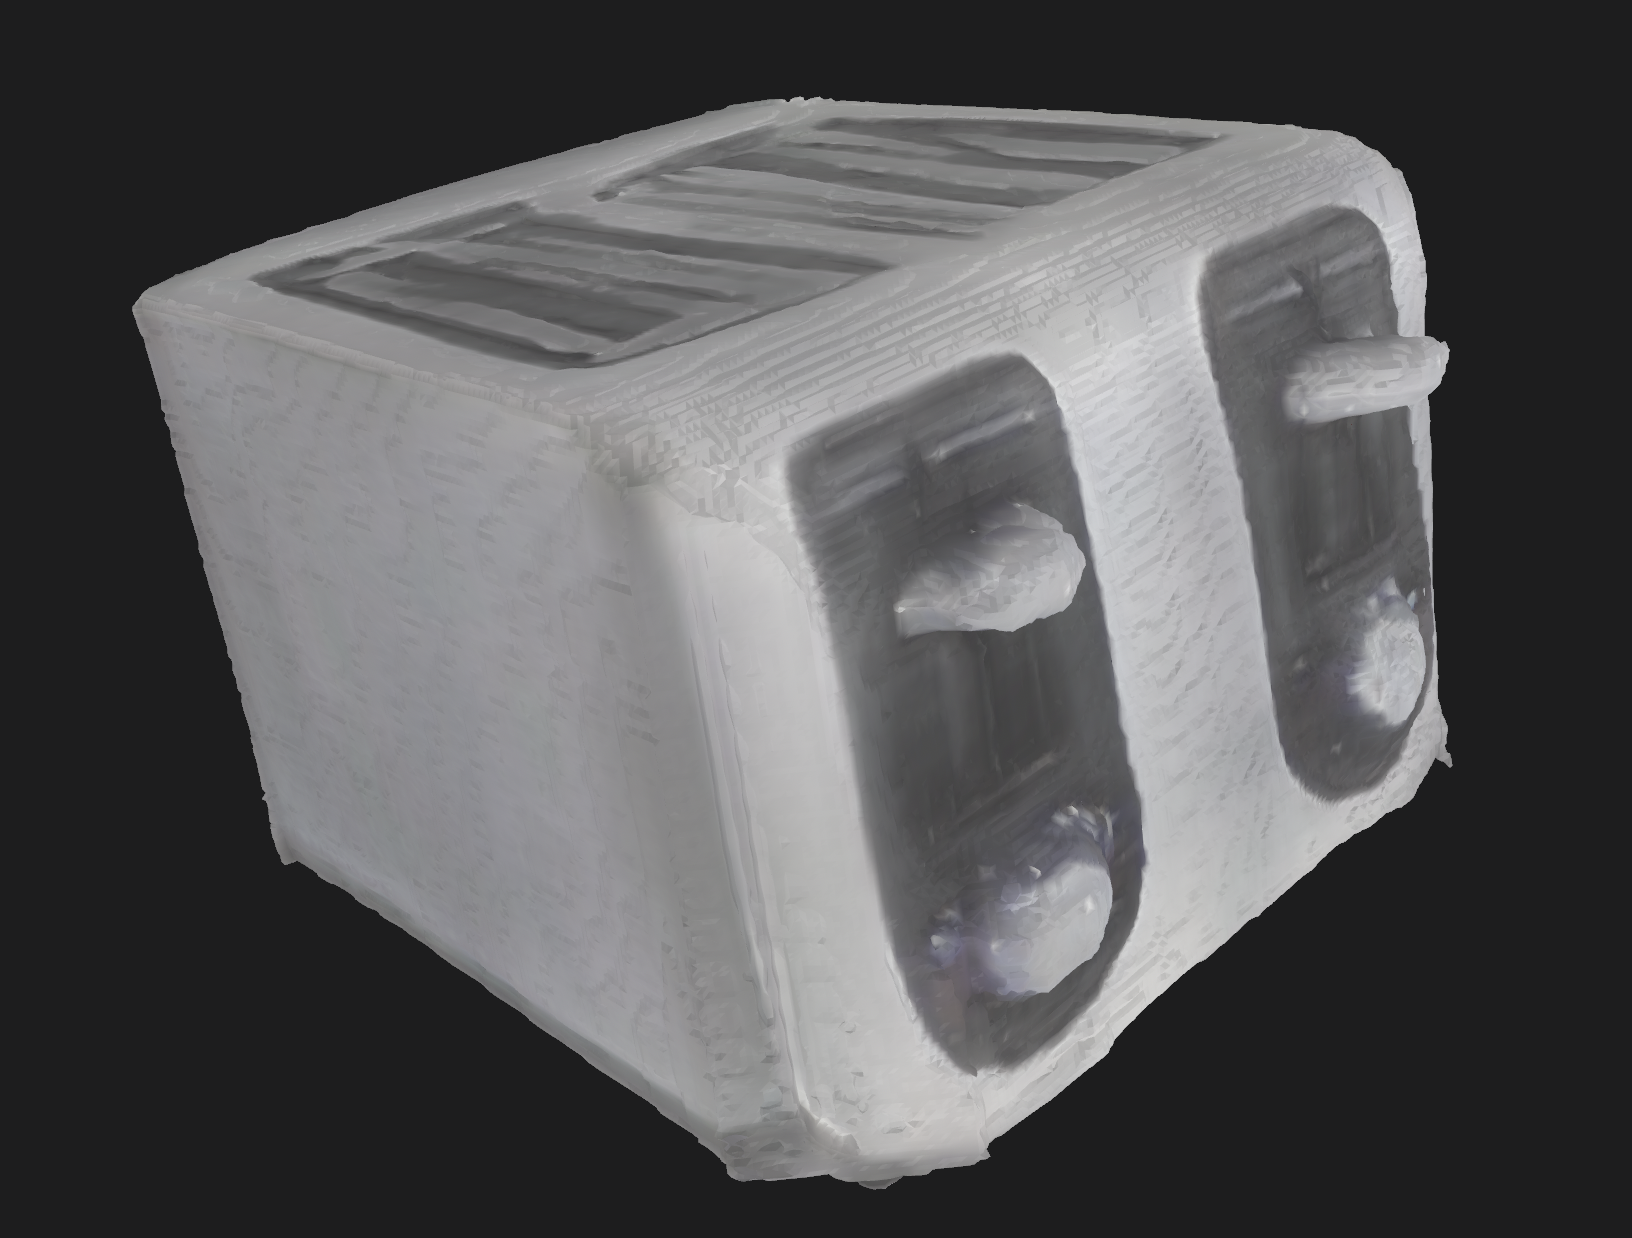
\includegraphics[height=2.2cm]{instantmesh_failure_case.png}\\[2pt]
        \scriptsize \textbf{Reflective surfaces}\\Diffusion hallucinates inconsistent novel views.
      \end{block}
    \column{0.32\textwidth}
      \begin{block}{\color{sf3dcolor}SF3D}
        \centering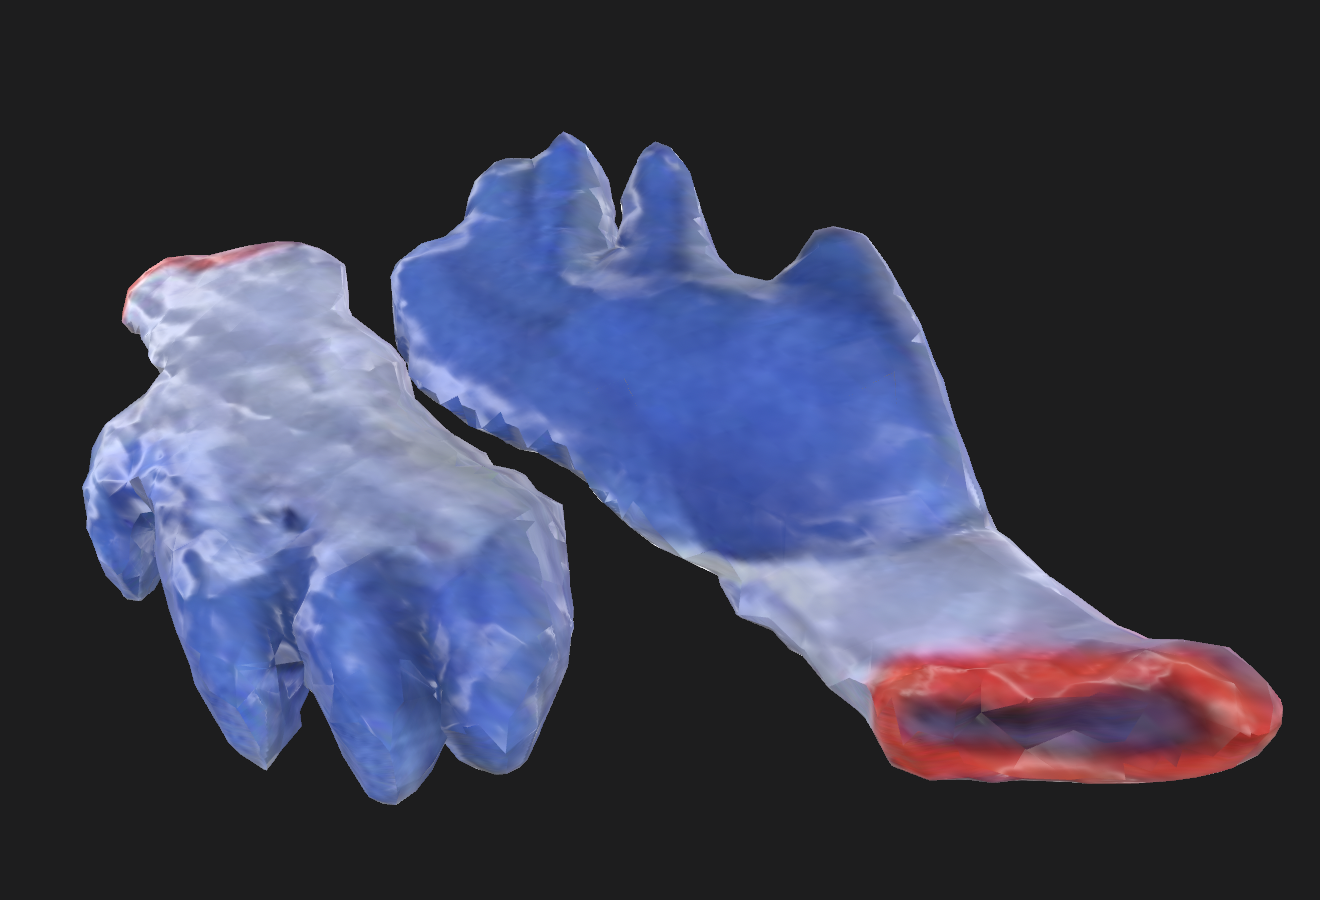
\includegraphics[height=2.2cm]{sfd3_failure_case.png}\\[2pt]
        \scriptsize \textbf{Spatially-varying material}\\MaterialNet predicts one global $(\rho, m)$.
      \end{block}
  \end{columns}

  \vspace{0.4em}
  \infocallout{Failures are \emph{architectural}, not random. They line up with the metrics on the previous slides.}
  \note{%
    These three failure modes are predictable from the
    architecture. TripoSR's $64^2$ triplane resolution literally
    cannot represent thin geometry. InstantMesh's diffusion stage
    breaks on reflective surfaces because it gets photometrically
    inconsistent input. SF3D's MaterialNet predicts global
    material parameters and so cannot represent half-matte /
    half-glossy objects. Each failure links back to a specific
    metric column on the result slides.}
\end{frame}

% =============================================================
% DECISION GUIDE
% =============================================================
\begin{frame}{When to pick which method}

  \begin{columns}[T]
    \column{0.55\textwidth}
      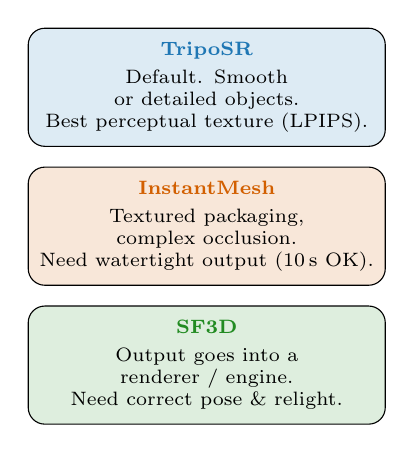
\begin{tikzpicture}[node distance=0.25cm]
        \node[draw, rounded corners=6pt, fill=tripocolor!15, minimum width=4.5cm,
              minimum height=1.5cm, font=\scriptsize, align=center,
              text width=4.3cm] (t)
          {\textcolor{tripocolor}{\textbf{TripoSR}}\\[2pt]
           Default. Smooth or detailed objects.\\
           Best perceptual texture (LPIPS).};
        \node[draw, rounded corners=6pt, fill=instantcolor!15, minimum width=4.5cm,
              minimum height=1.5cm, font=\scriptsize, align=center,
              text width=4.3cm, below=of t] (i)
          {\textcolor{instantcolor}{\textbf{InstantMesh}}\\[2pt]
           Textured packaging, complex occlusion.\\
           Need watertight output (10\,s OK).};
        \node[draw, rounded corners=6pt, fill=sf3dcolor!15, minimum width=4.5cm,
              minimum height=1.5cm, font=\scriptsize, align=center,
              text width=4.3cm, below=of i] (s)
          {\textcolor{sf3dcolor}{\textbf{SF3D}}\\[2pt]
           Output goes into a renderer / engine.\\
           Need correct pose \& relight.};
      \end{tikzpicture}

    \column{0.42\textwidth}
      \begin{alertblock}{Open problems (all three)}
        \scriptsize
        \begin{itemize}
          \item Transparent / reflective objects
          \item Wiry / thin geometry
          \item Spatially-varying materials
          \item Strict tolerance ($\tau{<}1\,\%$): F-Score $\sim 0.1$
        \end{itemize}
      \end{alertblock}
  \end{columns}
  \note{%
    Decision guide derived from the numbers on the result slides.
    Default to TripoSR -- best on LPIPS and on most property cells.
    InstantMesh when you have textured packaging or complex
    occlusion or need a watertight output. SF3D when the asset
    will go directly into a renderer or game engine where the
    pose has to be right and the material has to be relit.
    Open problems are common to all three -- thin structures,
    reflective surfaces, varying materials.}
\end{frame}

% =============================================================
% TAKEAWAYS
% =============================================================
\begin{frame}{Takeaways}

  \begin{itemize}
    \item \textbf{No method dominates.} Each wins a different metric family.
    \item \textbf{Architecture predicts behaviour.} NeRF $\Rightarrow$ smooth; diffusion $\Rightarrow$ filled-in occlusions; PBR $\Rightarrow$ better pose.
    \item \textbf{Property type matters more than averages.} Pick the model from the object class.
    \item \textbf{Single-image 3-D is still hard at strict tolerance} (F@1\,\% $\leq$ 0.15).
  \end{itemize}

  \vspace{1.2em}
  \begin{center}
    \large Thank you.\par\vspace{2pt}
    \scriptsize Code, data labels, and reports: see the GitHub repository.
  \end{center}
  \note{%
    Final summary. The three findings I want the audience to
    leave with: (1) no method dominates -- each wins a metric
    family; (2) architecture predicts behaviour, so the picks are
    rational, not arbitrary; (3) property-type-based selection
    beats picking the average winner. And single-image 3-D is
    still far from solved at strict tolerance.}
\end{frame}

\end{document}
